The tool used in this work to achieve single-atom control is optical tweezers: by focussing a laser beam to a small enough spot it has been shown that under the right conditions, this trap can house at most one atom. 

\section{Loading Single Atoms}\label{sec:LoadingAtoms}

Single atom loading was first demonstrated by \cite{Schlosser2001}. 
Call the number of atoms in the tweezer $N$, \cite{Schlosser2002} suggested for the time-derivative of $N$ a model with contributions

\begin{equation}\label{LoadingTweezer}
	\frac{\text{d}N}{\text{d}t} = \alpha - \gamma N - \beta N(N-1)
\end{equation}

where the first term $\alpha$ is the loading rate or the amount of atoms entering the tweezer per second. 
Next, $\gamma$ is the atom loss as a result of collisions with the background gas. 
Lastly, $\gamma$ is a measure for the mainly 2 body loss as a result of light-assisted collisions.
3-body terms and higher are disregarded. 
In order to load single atoms, we must satisfy $\beta \gg \gamma$: the two-body collisions are dominant.
We can now look at two distinct scenarios:

\begin{itemize}
	\item Starting from 0 atoms in the tweezer: an additional atom entering will now load the tweezer to $N=1$. 
	
	\item Starting from $N=1$: when an additional atom is loaded, the atoms will immediately kick out each other because of the tiny tweezer volume and strong light intensity from the MOT beams. 
\end{itemize}

If the number of atoms at $t=0$ is larger than $N$, atoms will be lost in pairs until $N$ is either 0 or 1, after which the events above apply. 
Apparently, a loading event can lead to either 0 or 1 atom in the tweezer, both with $50\%$ probability. 
This is known as the collisional blockade effect. Experimentally demonstrated by \cite{Schlosser2001} and \cite{Schlosser2002} showed this effect to exits for 3 orders of magnitude in the loading rate $\alpha$.
Satisfying $\beta \gg \gamma$ can be done by keeping $\gamma$ to a minimum by going to the ultra high vacuum regime.
We intent to go to a pressure of the order of $10^{-10}$ mbar. In addition $\beta$ is maximized by going to high light-intensities and small trapping volumes. 
The remainder of this chapter is dedicated on how to minimize this trapping volume.

\section{Diffraction Limit}

The smallest achievable spot size is governed by the diffraction limit, which states that because light is a wave, it is impossible to focus down to an infinitely small spot even in the absence of aberrations.
Diffraction is elegantly described by Fourier optics \cite{Goodman2005}. 
We derive a result used throughout this work here.

\begin{mdframed}
    \subsection*{Intermezzo Fourier Optics}
    
    As we use the objective to make a tweezer, light is impinging on its back aperture. 
    We call its complex amplitude $U(x',y')$ and define the aperture at $z = 0$ on the optical axis.
    After the aperture, light will show diffraction. 
    An elegant description is provided by scalar diffraction theory.
    We will not repeat a full derivation here but we can refer the reader to \cite{Goodman2005}.
    Consider the Fresnel diffracion integral in cartesian coordinates. 
    After the aperture, the complex amplitude $U$ distribution is:
    
    \begin{equation}\label{eq:FresnelDiffraction}
        U(x,y,z) = 
        \frac{e^{ikz}}{i \lambda z} \iint_{-\infty}^{\infty} U(x',y',0) \exp{\frac{ik}{2z}} \exp{\left[(x-x')^2+(y-y')^2\right]} dx'dy'.
    \end{equation}
    
    In \cref{eq:FresnelDiffraction}, $\lambda$ is the wavelength, $k=2\pi/\lambda$ the wavenumber.
    In this thesis, we are usually not immediately interested in describing the light in the the near field of the aperture, but in the far-field. 
    More formally, the following needs to apply:
    
    \begin{equation}\label{eq:FraunhoferCriterion}
        z \gg k R^2/2,
    \end{equation}
    
    where $R$ is the maximum distance from the aperture to the optical axis. 
    While this criterion is in practice not met, it does hold in the focal point of a lens, because a lens projects an image in infinity to its focal length $f$. 
    Inserting \cref{eq:FraunhoferCriterion} in \cref{eq:FresnelDiffraction} yields:
    
    \begin{equation}\label{eq:FraunhoferDiffraction}
        U(x, y, z)=\frac{e^{i k z} e^{i k\left(x^{2}+y^{2}\right)/2}}{i \lambda z} \iint_{-\infty}^{\infty} U(x', y') \exp \left[\frac{-ik}{z}(x x'+y y')\right] dx' dy'
    \end{equation}. 
    
    This equation relates the field in the focus point point of the lens $U(x,y)$ to the field at the lens $U(x',y')$. 
    Contributins outside of the apeture can be discarded, and in practice we are not too intersted in the phase factor in front, such that we have
    
    \begin{equation}\label{eq:FraunhoferSimplified}
        U(x,y,z) \propto 
        \iint_{\text{aperture}} U(x',y') \exp{\left[- \frac{ik}{z}(xx'+yy')\right]}dx'dy'
    \end{equation}
    
    We recognize in \cref{eq:FraunhoferDiffraction} the spatial Fourier transform, in both $x$ and $y$ with respectively the frequencies $f_x = x/\lambda z$ and $f_y = y/\lambda z$, which is a result we will use later in this work. \cref{eq:FraunhoferDiffraction} is the Fraunhofer diffraction integral.
\end{mdframed}

 In this work, we are mostly concerned with circularly shaped apertures, for which a description in cylindrical coordinates is more natural.
 Ignoring the phase factor in front of the integral:

\begin{equation}\label{eq:FraunhoferRTheta}
    U(r,\theta, z) \propto \iint_{\text{aperture}} U(r') \exp{\left[
    -\frac{i k r r'}{z} \cos{(\theta-\theta')} 
    \right]}r'dr'd\theta'
\end{equation}

Using the integral definition of the Bessel function of the first kind\footnote{$J_0(x) = \frac{1}{2\pi} \int_0^{2\pi} \exp{(i x \cos{\alpha})} d\alpha$} we write \cref{eq:FraunhoferRTheta} as 

\begin{equation}\label{eq:FourierBessel}
    U(r,z) \propto 2\pi \int_0^{\infty} U(r') J_0\left( \frac{k r r'}{z}\right) r'dr'
\end{equation}

\cref{eq:FourierBessel} is the Fourier-Bessel or Hankel transform.
Now that the general formula has been derived, will make the problem more specific by introducing some parameters. 
In practice, we are interested in the focus point of the lens around $z \approx f$. 
We send a Gausian beam through the lens with aperture radius $R$ such that for $r' <R$ we have $U(r')=e^{-r'^2/w_i^2}$ and $U(r'>R)=0$.
Substituting in \cref{eq:FourierBessel} yields

\begin{equation}\label{eq:FourierBesselAperture}
    U(r) \propto \int_0^R e^{-r'^2/w_i^2} J_0\left(\frac{k r r'}{f}\right)r'dr'
\end{equation}

\cref{eq:FourierBesselAperture} is analytically solvable for specific cases.
Letting $w_i/R$ go to infinity, which is to treat the incident Gaussian beam as a plane wave, we can neglect the exponential term in \cref{eq:FourierBesselAperture}. 
The integral is now tractable, yielding for the field amplitude

\begin{equation}\label{eq:AiryField}
    U(r) \propto \frac{f}{kRr} J_1\left(\frac{k R r}{f}\right)
\end{equation}

Taking the absolute value squared and normalizing yields the \ac{PSF}:

\begin{equation}\label{eq:NormalizedPSF}
    \frac{I}{I_0} = \left[
    \frac{2J_1(k r R/f)}{k r R/f}
    \right]^2
\end{equation}

\begin{figure}
    \centering
    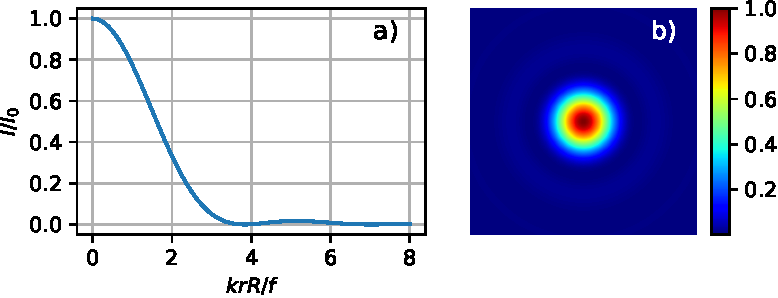
\includegraphics[width = 0.8\linewidth]{figures/AiryDisk.pdf}
    \caption{\textbf{a)} Normalized intensity of the perfect \ac{PSF} as a function of the azimuthal coordinate $r$ normalized in terms of units $f / kR$.
    \textbf{b) }2D plot of the Airy disk.  }
    \label{fig:AiryPlots}
\end{figure}

The point spread function of a circular aperture is shown in \cref{fig:AiryPlots}. 
Solving for the first zero of \cref{eq:NormalizedPSF}, and introducing under paraxial approximation the \ac{NA}: $\text{NA} \approx R/f$ yields for this radius 

\begin{equation}\label{eq:Abbe}
    d_1 = 0.61 \frac{\lambdaup}{\text{NA}}
\end{equation}

This result is known as the Abbe limit or diffraction limit \cite{Hecht2002} and it is the smallest feature the imaging system can produce. 
To minimize the \ac{PSF} we can thus increase the numerical aperture of our imaging system. 
In practice, often the side-rings of the Airy feature are not that clearly visible because of aberrations and it turns out the pattern is often better described by a Gaussian beam. 

\mbox{}\par
\begin{mdframed}
    \subsection*{Intermezzo Gaussian Beams}\label{sec:GaussianBeams}
    
    Optical tweezer are in essence tightly focused laser beams. We will briefly revisit the description of the commonly used laser beam because it is used throughout this work.
    Starting from Maxwell equations, one can derive under paraxial approximation a description of the transverse electromagnetic mode (TEM\textsubscript{00}) \cite{Leeuwen2017} for the electric field $E$.
    This Gaussian beam is most conveniently written down in cylindrical coordinates $\{r,z\}$:
    
    \begin{equation}\label{eq:GaussianBeam}
    	E(r,z) = \frac{w_0}{w(z)} \exp{\left(\frac{-r^2}{w^2(z)}\right)} \exp{\left[-ikz-i\frac{kr^2}{2R(z)} - i\psi(z)\right]},
    \end{equation}
    
    with parameters
    
    \begin{equation}\label{eq:GaussianBeamParameters}
    	k = \frac{2\pi}{\lambdaup}, \quad 
    	w(z) = \sqrt{w_0 + \frac{z^2}{z_R^2}}, \quad \text{and} \quad
    	R(z) = z \left(1 + \frac{z^2}{z_R^2}\right).
    \end{equation}
    
    Respectively, the wave number in terms of the wavelength $\lambdaup$, the beam waist, the radius where the field drops $1/e$ in terms of $w(z)\equiv w_0$ and $R(z)$ is the wavefront curvature. 
    Finally $\psi(z)$ is an extra phase term originating from the curvature of the wavefront known as the Gouy phase.
    We find the intensity of the Gaussian beam by taking the absolute value squared:
    
    \begin{equation}\label{eq:GaussianBeamIntensity}
    	I(r,z) = I_0 \frac{w_0^2}{w^2(z)} \exp{\left(\frac{-2r^2}{w^2(z)}\right)}
    \end{equation}
    
    A sketch of a Gaussian beam profile is given in \cref{fig:GaussianBeam}, showing the $1/e$ field radius, or $1/e^2$ intensity radius $w_0$ and the Rayleigh range or depth of focus $z_R$. 
    
    \vspace*{3mm}
    \centering
        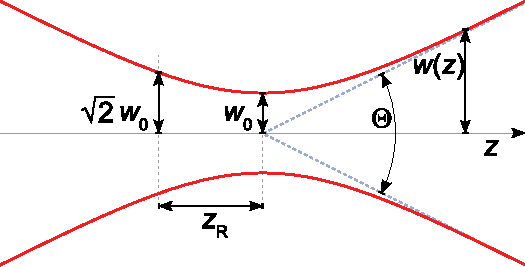
\includegraphics[width=0.4\linewidth]{figures/GaussianBeam.pdf}
        \captionof{figure}{Gaussian beam profile and some key parameters used in this work, the beam waist $w_0$ and Rayleigh range $z_R$. 
        Figure adapted from \cite{Hermans2009}.}
        \label{fig:GaussianBeam}
\end{mdframed}

Fitting this Gaussian as closesly as possible to an Airy pattern, it can be shown that the waist is \cite{Zhang2007}

\begin{equation}\label{GaussianAiryFit}
    w = 0.42 \frac{\lambdaup}{\text{NA}}
\end{equation}
 
If our waist is at this limit, we say the system is diffraction-limited, that is limited by the wave nature of light and not by aberrations or imperfections in the system. 
In practice, this is unachievable and other definitions like the Strehl ratio are used \cite{Sortais2007}, but that definition will not be used in this work. 

\section{Making the Tweezer}

So to minimize the trapping volume, we need the highest possible numerical aperture. But there are more demands our lens should satisfy: the \ac{MOT} and subsequent \ac{ODT} are made in a vacuum chamber so the beam traverse a vacuum viewport. This requires

\begin{enumerate}
    \item Ultra-long working distance (the distance between the trap and the lens). For a single lens, this is equivalent to the focal length of course, though for a compound lens this is a bit more complicated. 
    
    \item Glass-thickness compensation. The relatively thick vacuum viewport will introduce significant (spherical) aberrations for high NA and therefore big angles. It is possible to correct for this by having an additional lens which will counteract this.
\end{enumerate}

To achieve this, we chose the G Plan Apo microscope objective from \textit{Mitutoyo}, as also used by \cite{Manuel2016,Ebadi2021}. 
This is an infinity-corrected objective, meaning light collected in its focussed is imaged at infinity (parallel beam) and an additional field lens is used to focus this image, such that the magnification is 

\begin{equation}\label{eq:InfinityMagnification}
    M = \frac{f_2}{f_1},
\end{equation}

where $f_2$ is the focal length of the field lens and $f_1$ the equivalent focal length of the objective\footnote{For a compound microscope objective, equivalent focal length means the focal length the objective would have when replaced by a single lens.}. Relevant specifications of the objective are shown in \cref{table:MitutoyoSpecs}. 
From compound objectives, the equivalent focal length is defined in terms of the \ac{NA} and the equivalent focal length from we can deduce a back aperture radius of $R = f_1 \text{NA} = 2$ mm. 

\begin{table}[h]
    \centering
    \caption{Key specifications of the objective from manufacterer Mitutoyo.}
    \label{table:MitutoyoSpecs}
    \begin{tabular}{l | l}
        \textbf{Specification}       & \textbf{Value} \\ \hline 
        NA                           & 0.5            \\ \hline
        Glass thickness compensation\footnote{We assume 3.5 mm of N-BK7 glass is used here, which has a slightly different refractive index than quartz for example.} & 3.5 mm         \\ \hline
        Equivalent focal length      & 4 mm           \\ \hline
        Working distance             & 15.08 mm      
    \end{tabular}
\end{table}

Because this objective was designed with visible wavelenghts in mind, it is probable that all of the lenses inside it are coated with a reflection coating that does not work well for the 800 nm regime. 
This is indeed the case, as we measured the tranmission of the objective to be just $(47 \pm 3)\%$ at 820 nm. We will therefore lose a significant of laser power. 
But this is not the only source of laser power loss: in producing the Airy pattern we assumed plane wave illumination, but in practice laser beams have Gausian shape. 
As a result, when working with a beam significantly larger than the back aperture this excess power is lost. 
Assuming the beam is aligned with the center of the aperture, the power tranmission $P/P_0$ as a function of the incident waist $w_i$ is

\begin{equation}\label{eq:FracPowerCircular}
    P/P_0 = 1 - e^{-2w_i^2/R^2}
\end{equation}

which tends to zero for very wide beams (plane waves). To find the optimum waist we will have a look at what the theoretical potential will be as a result from the tweezer beam, but a priori we know the resulting potential will be something in between a Gaussian beam and an Airy pattern. 

\section{Tweezer Potential}

From \cref{eq:Stark} we know that the potential of the tweezer is proportional to the light intensity. Assuming a Gaussian tweezer beam, the potential $U$ in cylindrical coordinates will be roughly (\cref{eq:GaussianBeam,eq:GaussianBeamParameters}).

\begin{equation}\label{eq:GaussianPotential}
    U(r,z)=\frac{-U_{0}}{1+z^{2} / z_{R}^{2}} \exp \left(\frac{-2 r^{2}}{w_{0}^{2}\left(1+z^{2} / z_{R}^{2}\right)}\right)
\end{equation}

\cref{eq:GaussianPotential} is plotted in \cref{fig:GaussianPotential} for normalized radial coordinate $r/w_0$ as well as longitudinal coordinate $z_R$. 
This is not to scale: the Rayleigh range $z_R$ is typically bigger than the waist $w_0$.
Assuming a Gaussian is justified because near the center, an Airy disk and Gaussian beam are nearly identical.
We are interested in potentials much deeper than the temperature of the atoms, such that the atoms will mostly occupy the bottom of the tweezer. 
Taylor expanding \cref{eq:GaussianPotential} around $(r,z)=(0,0)$ to second order yields 

\begin{figure}
    \centering
    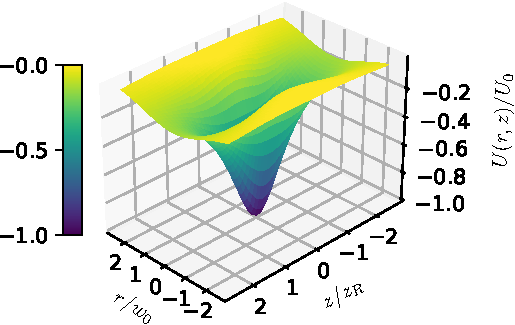
\includegraphics[width=.56\linewidth]{figures/GaussianPotential.pdf}
    \caption{Normalized potential from a Gaussian intensity shape. The independent coordinates are the normalized cylindrical coordiantes $r/w_0$ and $z/z_R$.}
    \label{fig:GaussianPotential}
\end{figure}

\begin{equation}\label{eq:ApproximateGaussianPotential}
    U(r,z) \sim -U_0 - 2U_0 \frac{r^2}{w_0^2} - 2U_0 \frac{z^2}{z_R^2}
\end{equation}

For this harmonic potential, one can compute the harmonic oscillation frequencies 

\begin{equation}
    \omega_r = 2\left(\frac{U_0}{m w_0^2}\right)^{1/2}, \quad
    \omega_z= \left(\frac{2 U_0}{m z_R^2}\right)^{1/2}
\end{equation}

Because $z_R > w_0$, the longitudinal oscillation frequency is lower than the radial frequency.

% We follow \cite{Madjarov2021} and look at two extreme cases for \cref{eq:FourierBesselAperture,eq:FracPowerCircular}


%     \item $w_i \ll R$. The waist is much smaller than the aperture, according to \cref{FracPowerCircular} we have maximum power efficiency. We let the integration boundary run to infinity and using a Hankel tranform pair\footnote{$F_0(k) = \int_0^{\infty} e^{-1/2 a^2 r^2} J_0(k r)r dr = \frac{1}{a^2} e^{-\frac{k^2}{2a^2}}$} find 

% \begin{equation}
%     U(r) \propto \frac{w_i^2}{2} \exp{\left(\frac{-k^2w_i^2 r^2}{2f^2}\right)}.
% \end{equation}
%         
%     The result is a Gaussian, but with a modified waist of $\lambdaup f / \pi w_0$.  The result is similar to Gaussian apodization, where the size lobes of the Airy function are gone. 
% \end{enumerate}





We can discuss the two extreme cases again:

\begin{enumerate}
    \item For the case $w_i \gg R$, the power transmission will be low and therefore also the trap depth $-U_0$.
    \item For $w_i \ll R$, the waist of the resulting Gaussian in radial and longitudal directions $w_0$ and $z_R$ will increase, which is undesired. Because the total amount of power in the trap is fixed, because of normalization the trap depth is lower as well. 
\end{enumerate}





\section{Measuring the Tweezer potential}

We would like to measure tweezer potential of our high NA objective. We could use the objective to look at a pinhole and record its point spread function. However, in practice we don not send a plane wave but a Gaussian beam through the objective. As a result of this, two things are different \cite{Sortais2007}

\begin{itemize}
    \item As a result of apodization, the Airy rings will be damped. 
    \item The tweezer waist will be slightly broader: $\approx 9\%$.
\end{itemize}

In order to experimentally determine these effects, we send a Gaussian beam with a waist equal to the aperture radius through the microscope objective. We follow \cite{Baumgaertner2017}: we use another microscope objective to look into the tweezer waist of the Mitutoyo. But in order to avoid further convolution with the point spread function of the second objective, we use a higher NA for the second objective \footnote{Newport M-60X 0.85 NA objective}. Because there is no glass cell, this objective does not need ultra-long working distance so this higher NA is no problem. In order to record the 3D PSF, the tweezer is moved using a picomotor attenuator. 

\subsection{Calibration Imaging System}

The magnification of the Newport objective of 60X is only specified when used in a microscope with standard tube length distance, because it is finite conjugate corrected. Because our CCD is not exactly at the distance where normally the eyepiece of the microscope would be, we have to calibrate its magnification. We do this using a high resolution target \footnote{Edmund Optics high resolution microscope target.} 

We illuminate the target with an incoherent light source (LED) because the laser would cause interference from the different lines. We neglect the slightly different focus point from the Newport objective for our laser frequency compared to white light. 

\begin{figure}
    \centering
    \includegraphics[width = 2.5in]{figures/linespacing.pdf}
    \caption{Image from the resolution target illuminated showing lines spaced by 45 lines per mm.}
    \label{fig:resolutionTarget}
\end{figure}

To detect the edges in \cref{fig:resolutionTarget}, we use an edge detection algorithm script that averages over all vertical pixels, blurs using a Gaussian to surpress noise and computes the derivative. When the derivative surpasses a set threshhold we define it as an edge. The magnification was found to be $(50.3\pm0.5)$X. This is smaller than the specified 60X, which we attribute to an incorrect tube length distance. 

\subsection{Picomotor Attenuators}

The target was also used to calibrate the picomotor attenuator. We measured over the maximum available amount of lines of similar spacing of 5 using 4000 picomotor steps, and correcting for the shift in camera found a step size of $20.3\pm0.1$ nm, which matched exactly with the specifications of the piezo-attenuator for the given load. This result will be used in the 3D scanning of the tweezers. 

The stage we used is 8081-M 5-axis motorized tilt aligner from Newport. There is no reason here to use a 5-axis stage because we only need translation in one direction, but we will use this stage later to mount the objective in the final setup. To drive this stage, we used a set of Newport 8742 controllers in daisy-chain configuration. 



